\documentclass[a4paper,12pt]{article}

\usepackage{cmap}          % поиск в PDF
\usepackage{mathtext}         % русские буквы в формулах
\usepackage[T2A]{fontenc}      % кодировка
\usepackage[utf8]{inputenc}      % кодировка исходного текста
\usepackage[english,russian]{babel}  % локализация и переносы
\usepackage[left=2cm,right=2cm,top=2cm,bottom=2cm]{geometry}
\usepackage{amsfonts,amssymb,amsthm,mathtools} % AMS
\usepackage{amsmath}
\usepackage{icomma} % "Умная" запятая: $0,2$ --- число, $0, 2$
\usepackage{graphicx}
\usepackage{wrapfig} % картинка в тектсе
\usepackage{caption} % убирается номер у подписей caption*{}
\usepackage{csquotes} % цитаты
\usepackage{multirow} % для жестких таблиц
\usepackage{hhline}
\usepackage{indentfirst} % абзацный отступ после section
\usepackage{epigraph} % эпиграф
\usepackage{tikz}
\usepackage{pgfplots}
\usepackage[export]{adjustbox}
\usepackage{tabularx}
\usepackage{float}
\usepackage{longtable}

\begin{document}
\setcounter{section}{4}
\section{Результаты измерений}

\subsection*{Определение момента инерции ротора}
\textbf{Момент инерции цилиндра} можно вычислить по следующей формуле:

$$I_\text{ц} = \frac{1}{2}m_\text{ц}\left( \frac{d_\text{ц}}{2}\right)^2$$

где $ m_\text{ц} = (1,619 \pm 0,0003) $ кг -- масса цилиндра, $ d_\text{ц} = (0,078 \pm 0,0001) $ м -- его диаметр.

$$I_\text{ц} = 0,00123 \text{ кг} \cdot \text{м}^2$$
Погрешность определения момента инерции равна 
$$\Delta I_\text{ц} = I_\text{ц}\sqrt{\left( \frac{\Delta m_\text{ц}}{m_\text{ц}} \right)^2 + \left(2 \frac{\Delta d_\text{ц}}{d_\text{ц}} \right)^2 } \approx 0,000003 \text{ кг} \cdot \text{м}^2$$

$$I_\text{ц} = \left(0,001230 \pm 0,000003 \right) \text{ кг} \cdot \text{м}^2$$

Далее вычислим \textbf{период крутильных колебаний цилиндра}, подвесив его на проволоке. Померим время его 5 колебаний.

\begin{table}[!ht]
    \centering
    \begin{tabular}{|l|l|l|l|}
    \hline
        N & $T_5,$ с & T, с \\ \hline
        1 & 20,32 & 4,064 \\ \hline
        2 & 20,03 & 4,006 \\ \hline
        3 & 20,11 & 4,022 \\ \hline
    \end{tabular}
\end{table}
Тогда среднее время колебаний равно $T = 4,03$ c. Определим случайную погрешность по формуле
$$\sigma^{\text{сл}}_T = \sqrt{\frac{1}{N_\text{оп}} \sum_{i = 1}^{N_\text{оп}} \left(T_i - \langle T \rangle \right)^2} = 0.03 \text{ c}$$

Полная погрешность может быть вычислена по формуле, где $\Delta_\text{сек} = 0.5$ с - время реакции человека:
$$ \Delta T_ц = \sqrt{\left( \sigma^\text{сл}_T \right)^2 + \left(\frac{\Delta_\text{сек}}{N}  \right)^2  } = 0,104 \text{ c}$$
$$ T_\text{ц} = \left( 4,030 \pm 0,104\right) \text{ с} $$

Вычислим \textbf{период крутильных колебаний ротора}. Померим время его 7 колебаний.
\begin{table}[!ht]
    \centering
    \begin{tabular}{|l|l|l|l|}
    \hline
        N & $T_7,$ с & T, с \\ \hline
        1 & 22,21 & 3,173 \\ \hline
        2 & 22,42 & 3,203 \\ \hline
        3 & 22,48 & 3,211 \\ \hline
    \end{tabular}
\end{table}
\par Тогда среднее время колебаний равно $T = 3,196$ c. Аналогично посчитаем погрешность . Тогда $\sigma^{\text{сл}}_T = 0,016$ c.
$$ \Delta T_0 = \sqrt{\left( \sigma^\text{сл}_T \right)^2 + \left(\frac{\Delta_\text{сек}}{N}  \right)^2  } = 0,073 \text{ c}$$
$$ T_0 = \left( 3,196 \pm 0,073\right) \text{ с} $$

Тогда момент инерции ротора равен:
$$I_0=I_\text{ц}\frac{T_0^2}{T_\text{ц}^2} = 0,00077 \text{ кг} \cdot \text{м}^2.$$
Погрешность вычисления момента инерции ротора гироскопа можно вычислить по формуле:
$$\Delta I_0 = I_0\sqrt{\left( \varepsilon_{I_\text{ц}} \right)^2 +\left( 2 \varepsilon_{T_0} \right)^2 + \left(2 \varepsilon_{T_\text{ц}} \right)^2} \approx 0,00005 \text{ кг} \cdot \text{м}^2.$$
В итоге получаем:
$$I_0 = \left( 0,00077 \pm 0,00005 \right) \text{ кг} \cdot \text{м}^2$$


\subsection*{Определение частоты вращения ротора}
Для определения частоты вращения ротора гироскопа будем исследовать зависимость скорости прецессии гироскопа в зависимости от момента силы, действующей на его ось. Результаты измерений представлены в таблице.


\begin{table}[!ht]
    \centering
    \begin{tabular}{|c|c|c|c|c|c|c|c|c|c|}
    \hline
        $N$ & $m$, кг & $M \text{, Н} \cdot м$  & $\Delta M \text{, Н} \cdot м $ & $T_1$, c & $T_2$, c & $T$, c & $\varepsilon_T$ & $\Omega \text{, c}^\text{-1}$ & $\Delta \Omega  \text{, c}^\text{-1}$  \\ \hline
        1 & 0,342 &  0,3988 & 0,0004 & 29,66 & 29,69 & 29,68 & 0,034 & 0,212 & 0,007  \\ \hline
        2 & 0,274 & 0,3195 & 0,0003 & 36,56 & 37,28 & 36,92 & 0,027 & 0,170 & 0,005  \\ \hline
        3 & 0,220 & 0,2566 & 0,0003 & 45,73 & 44,8 & 45,27 & 0,022 & 0,139 & 0,003  \\ \hline
        4 & 0,179 & 0,2087 & 0,0002 & 56,89 & 57,1 & 57,00 & 0,018 & 0,110 & 0,002  \\ \hline
        5 & 0,142 & 0,1656 & 0,0002 & 71,24 & 72,3 & 71,77 & 0,014 & 0,088 & 0,001  \\ \hline
        6 & 0,093 & 0,1085 & 0,0002 & 108,23 & 107,11 & 107,67 & 0,009 & 0,058 & 0,001 \\ \hline
    \end{tabular}
\end{table}

Погрешность вычисления момента силы определяется следующим соотношением:
	

	$$\Delta M = M\sqrt{\left( \frac{\Delta_\text{вес}}{m} \right)^2 + \left( \frac{\Delta_\text{лин}}{l} \right)^2}$$
	Погрешность вычисления скорости прецессии равна:
		$$\Delta \Omega = \Omega \cdot \varepsilon_T$$
    По полученным данным построили график.

    $$\Omega = kM$$
    $$k = \frac{1}{I_0\omega_0}$$

    Коэффициент наклона прямой можно посчитать по МНК
    $$k = \frac{\langle M\Omega\rangle}{\langle M^2 \rangle} \approx 0,532 \text{ } \frac{1}{\text{Дж} \cdot \text{с}}$$

    Случайную погрешность определения $ k $ можно вычислить по следующей формуле:
    $$\sigma^\text{сл}_k = \frac{1}{\sqrt{N_\text{оп}-1}} \sqrt{\frac{\langle \Omega^2 \rangle}{\langle M^2 \rangle} - k^2} \approx 0,003 \text{ } \frac{1}{\text{Дж} \cdot \text{с}}$$

    Систематическую погрешность определения $ k $ можно вычислить следующим образом:
	
	$$\sigma^\text{сист}_k = k\sqrt{\left( \frac{\Delta M}{M} \right)^2+\left(\frac{\Delta \Omega}{\Omega} \right)^2} \approx 0,017 \text{ } \frac{1}{\text{Дж} \cdot \text{с}}$$

    Тогда полная погрешность определения $ k $ определяется следующим образом:

	$$\Delta k = \sqrt{\left( \sigma_k^\text{сл} \right)^2 + \left( \sigma_k^\text{сист} \right)^2  } \approx 0,018 \text{ } \frac{1}{\text{Дж} \cdot \text{с}}$$

    Тогда:
    $$k =\left( 0,532 \pm 0,018 \right) \frac{1}{\text{Дж} \cdot \text{с}} , \left( \varepsilon = 3,4 \% \right)$$

\begin{figure}[H]
    \centering
    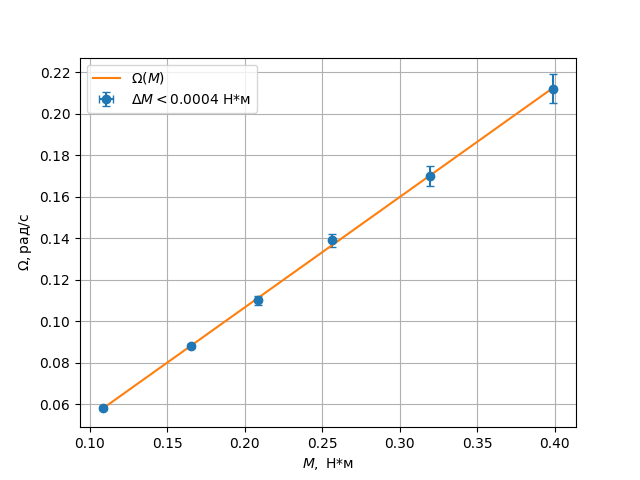
\includegraphics[width=0.9\textwidth]{graph.png}
    \caption{График зависимости скорости прецессии гироскопа от момента силы}
\end{figure}

    С помощью $ k $ можно вычислить угловую скорость вращения ротора гироскопа:
	
	$$\omega_0 = \frac{1}{I_0 k}$$

	Используя угловую скорость, можно определить частоту вращения ротора гироскопа:
	$$\nu = \frac{\omega_0}{2\pi} = \frac{1}{2\pi I_0 k } = 388 \text{ Гц}$$
	
    $$\Delta \nu = \nu \sqrt{\left( \frac{\Delta {I_0}}{I_0} \right)^2 + \left( \frac{\Delta k}{k} \right)^2} = 27 \text{ Гц}$$
   
	
	Таким образом, мы получили:
		 $$ \nu = \left( 388 \pm 27 \right) \text{ Гц}, \left( \varepsilon = 7,21 \% \right)   $$


\subsection*{Определение частоты вращения ротора гироскопа при помощи осциллографа}
Частоту измеряем по фигурам Лиссажу, получаемым на экране осциллографа, если на один вход подать исследуемую ЭДС, а на другой — переменное напряжение с хорошо прокалиброванного генератора. При совпадении частот на экране получится неподвижный эллипс.\\
	При настройке генератора сигнала на частоту \underline{$ \nu_0 = 386,5$ Гц} на экране осциллографа виден  неподвижный эллипс, следовательно эта частота сигнала совпадает с частотой вращения ротора гироскопа.

\subsection*{Оценка момента силы трения}

Для оценки силы трения будем измерять на какую высоту опустился груз за $t$

\begin{table}[!ht]
    \centering
    \begin{tabular}{|c|c|c|c|c|c|c|}
    \hline
        ~ & $N$ & $m$, кг & $T$, c & $h$, мм & $\Omega \text{ } \frac{рад}{с}$ & $М$, Н $\cdot \text{ м}^2$  \\ \hline
        ~ & 1 & 0,342 & 59,7 & 8 & 0,0107 & 0,0201  \\ \hline
        ~ & 2 & 0,274 & 110,0 & 9 & 0,0120 & 0,0226  \\ \hline
        ~ & 3 & 0,22 & 91,4 & 8 & 0,0107 & 0,0201  \\ \hline
        ~ & 4 & 0,179 & 115,2 & 8 & 0,0107 & 0,0201  \\ \hline
        ~ & 5 & 0,142 & 142,5 & 7 & 0,0094 & 0,0176  \\ \hline
        ~ & 6 & 0,093 & 108,5 & 6 & 0,0080 & 0,0151 \\ \hline
    \end{tabular}
\end{table}
$$M = \Omega I_0\omega_0 = \frac{\Omega}{k}$$
$$\varepsilon_\Omega = \varepsilon_h = \frac{1 \text{ мм}}{h} \text{ и тогда } \Delta M = M\sqrt{\varepsilon_k^2+\varepsilon_\Omega^2}$$
$$M_\text{ср} = 0,019 \pm 0,003 \text{ Н} \cdot \text{ м}^2$$


\section{Обсуждение результатов} 
В ходе работы мы определили практически частоту вращения ротора гироскопа. Она равна $ \nu = \left( 388 \pm 27 \right) \text{ Гц}$. Небольшое отклонение от измеренной частоты осциллографом $\nu = 386,5 \text{ Гц}$
Можно обусловить тем, что мы использовали основное приближение гироскопа. Так же свой вклад внесли погрешность коэффициента наклона прямой и измеренного момента инерции ротора гироскопа. 
Наибольшую погрешность в измерение момента инерции внесло измерение периодов $T_0$ и $T_ц$, а момент инерции цилиндра был измерен с большой точностью. А периоды имеют такую погрешность, потому что мы мерили время малого количества колебаний. Еще в формуле $I_0$ периоды стоят в квадрате, поэтому их относительная погрешность удваивается.
Теперь для погрешности коэф. наклона прямой. В нее основную погрешность внесло систематическая ошибка. Так как погрешность измерения времени равна полсекунды, а еще надо учесть случайную ошибку. Так же мы мерили время лишь одного периода. У момента была маленькая погрешность, так как масса и длина плеча была дана с большой точностью.
Оценка момента силы трения имеет довольно большую погрешность из за плохого измерения высоты, на которую опустился рычаг. Абсолютная ошибка равна 1 мм, а сама величина не больше 10 мм, поэтому относительная погрешность порядка десяти процентов.  

\section{Вывод}
В данной лабораторной работе мы: \par
\begin{enumerate}
    \item Научились работать с гироскопом.
    \item Узнали, как найти момент инерции тела сложной формы используя крутильные колебания и используя тело с известным моментом инерции. Момент инерции тела сложной формы вычисляется с помощью момента инерции тела с известным моментом инерции и отношений периодов в квадрате.
    \item Оценили момент силы трения в гироскопе
    \item Для того, чтобы увеличить точность измерения момента силы трения необходимо придумать способ, который будет точнее измерять на какую высоту опустился рычаг.
    \item Нашли частоту вращения ротора гироскопа с помощью его прецессии. 
    \item Для увеличения точности измерения частоты вращения необходимо мерить время большего числа оборотов. Например измерять время 5-7 оборотов. 
    \item Так же можно увеличить количество точек в графике, тогда уменьшится случайная ошибка. То есть провести измерения со всеми грузиками, которые были в оборудовании. 
    \item Проверили, что выполняется приближение гироскопа. Скорее всего, другие ошибки внесли большее отклонение в измерения.
    \item Измерили частоту вращения ротора при помощи осциллографа. Чтобы получить частоту, необходимо было получить совпадение частот на генераторе и на исследуемой ЭДС. При совпадении на экране появлялся неподвижный эллипс.
    
\end{enumerate}
\end{document}
